
\pagebreak
\section{Qualitätsmanagement konsultieren}

Das Thema Qualitätsmanagement ist in zwei Bereiche unterteilt: 

\vspace{\baselineskip}

\begin{itemize}
\item
\textbf{Qualitätsmanagement}: Sie können hier bestehende Dokumentationen (Prozesse, Richtlinien etc.) im CUBE PA einbinden.
\item
\textbf{Handbücher: }Sie haben die Möglichkeit gegliederte Dokumentationen wie Projekthandbücher etc. im CUBE PA zu erstellen.
\end{itemize}

\vspace{\baselineskip}

\subsection{Qualitätsmanagement}

Bestehende Dokumente können Sie im CUBE PA integrieren und auf diese Weise einem Projektteam zugänglich machen. Bitte beachten Sie, dass die Dokument-Verknüpfungen nur durch Administratoren vorgenommen werden können. Wenden Sie sich an Ihren CUBE PA Superuser oder per Email an den CUBE PA Support: {\color{red} cube.support@emchberger.ch}.

\subsubsection{Dokumente unter Qualitätsmanagement abrufen}

Wie folgt können Sie ein verknüpftes Dokument abrufen:

\vspace{\baselineskip}

\begin{wrapfigure}[9]{l}{6.5cm}   % [x] Wie manche Zeile soll sich um die Grafik "brechen"
  \vspace{-35pt}      % Grundwert war 20; mit 30 schön oben beim Text ausgerichtet
  \begin{center}
    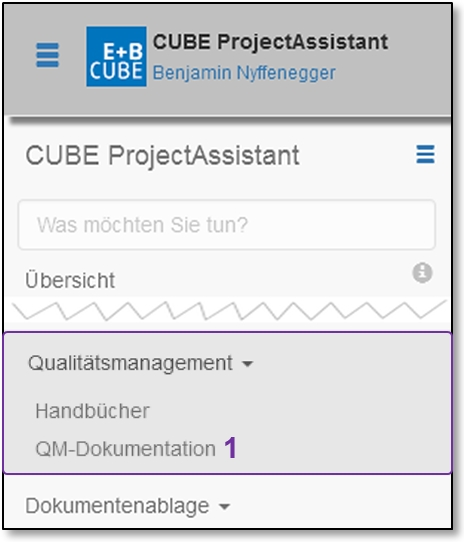
\includegraphics[width=1\linewidth]{../chapters/09_Qualitaetsmanagement/pictures/9-1_Menu_Qualitaetsmanagement.jpg}
  \end{center}
  \vspace{-20pt}
  \caption{Das Qualitätsmanagement verwenden}
  \vspace{-10pt}
\end{wrapfigure}

Wählen Sie im Menü links den Punkt 'Qualitätsmanagement' und hier in unserem Beispiel den Unterpunkt 'QM-Dokumentation' \col{(1)}.
 
\vspace{2cm} 

\textbf{Anmerkung:} Wenn Sie mehrere Dokumente verknüpft haben, werden diese alle unter dem Menüpunkt 'Qualitätsmanagement' angezeigt. Die Anzeigenamen können Sie selbst wählen (siehe dazu Kapitel \ref{bkm:Ref912000789}). \\

\pagebreak
Folgende Ansicht wird nun im rechten Fensterbereich angezeigt:

\begin{figure}[H]
\center{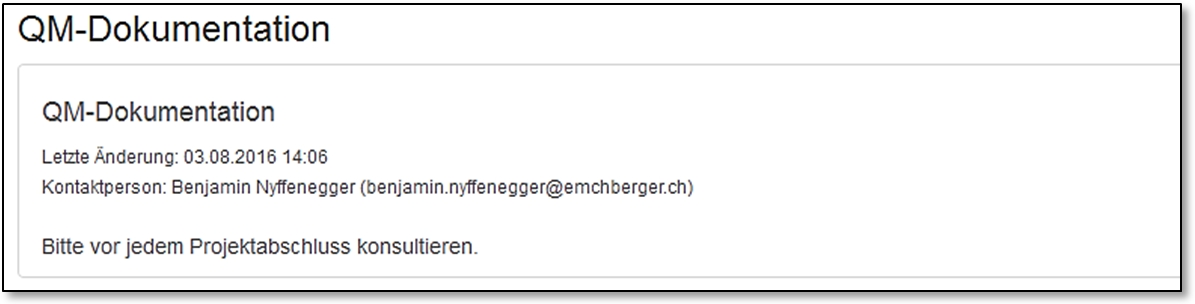
\includegraphics[width=1\linewidth]{../chapters/09_Qualitaetsmanagement/pictures/9-1_Verkn_Dokument.jpg}}
\caption{Ein verknüpftes Dokument öffnen}
% \label{fig:speciation}
\end{figure}

Sie sehen nun den Dokumentennamen und die dazugehörige Beschreibung. Zudem ist ersichtlich, wer für das Dokument verantwortlich ist und wann die letzte Änderung gemacht, respektive  das Dokument zuletzt hochgeladen wurden. Mit Klick in das umrahmte Feld können Sie nun das hinterlegte Dokument öffnen oder auf dem Computer speichern. Es wird ein weiterer Dialog angezeigt, welcher abhängig von dem verwendeten Browser ist.

\subsubsection{Dokumente unter Qualitätsmanagement verknüpfen}
\label{bkm:Ref912000789}

Dieser Vorgang erfordert höhere Rechte im CUBE PA. Kontaktieren Sie Ihren CUBE PA Superuser oder wenden Sie sich per Email an den CUBE PA Support: {\color{red} cube.support@emchberger.ch}.

\vspace{\baselineskip}

Soll ein (oder ein weiteres) Dokument unter 'Qualitätsmanagement' verknüpft werden, gehen Sie wie folgt vor:

\vspace{\baselineskip}

\textbf{1. Schritt: 'Anzeigedatentypen' erstellen}

Zuerst muss unter dem Menüpunkt links 'Konfigurationen' und dem Unterpunkt 'Anzeigedatentypen' ein neuer Begriff für das Menü erstellt werden (In unserem Beispiel wurde dazu der Begriff 'QM-Dokumentation' gewählt). Klicken Sie auf den Unterpunkt 'Anzeigedatentypen'. Sie sehen nun die Übersicht aller bereits erstellter Anzeigedatentypen und haben hier die Möglichkeit mittels dem Plussymbol 
\includegraphics[height=12pt]{/Icons/Plussymbol.jpg} \col{(1)} ein neuer Eintrag zu erstellen:

\begin{figure}[H]
\center{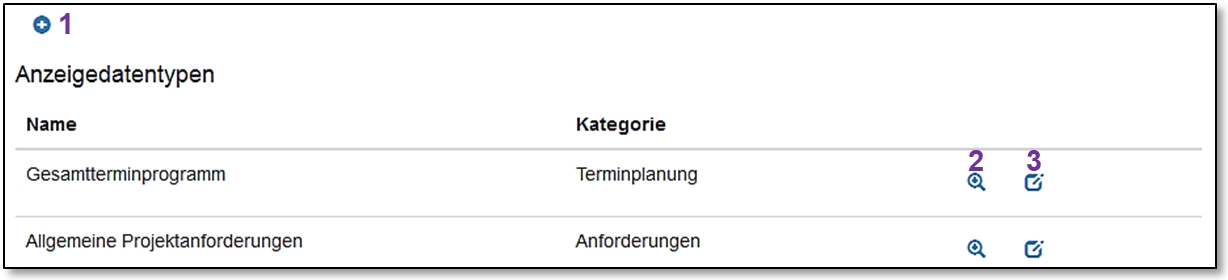
\includegraphics[width=1\linewidth]{../chapters/09_Qualitaetsmanagement/pictures/9-1-1_Anzeigedatentypen_Uebersicht.jpg}}
\caption{Anzeigedatentypen Übersicht}
% \label{fig:speciation}
\end{figure}

Mit der Lupe 
\includegraphics[height=12pt]{/Icons/Lupe.jpg} \col{(2)} können Sie sich bestehende Einträge ansehen, mit dem Bearbeitungssymbol 
\includegraphics[height=12pt]{/Icons/Bearbeiten.jpg} \col{(3)} können Sie einen bestehenden Eintrag bearbeiten. Mit Klick auf das Plussymbol 
\includegraphics[height=12pt]{/Icons/Plussymbol.jpg} \col{(1)} können folgende Eingaben und Einstellungen gemacht werden:

\begin{figure}[H]
\center{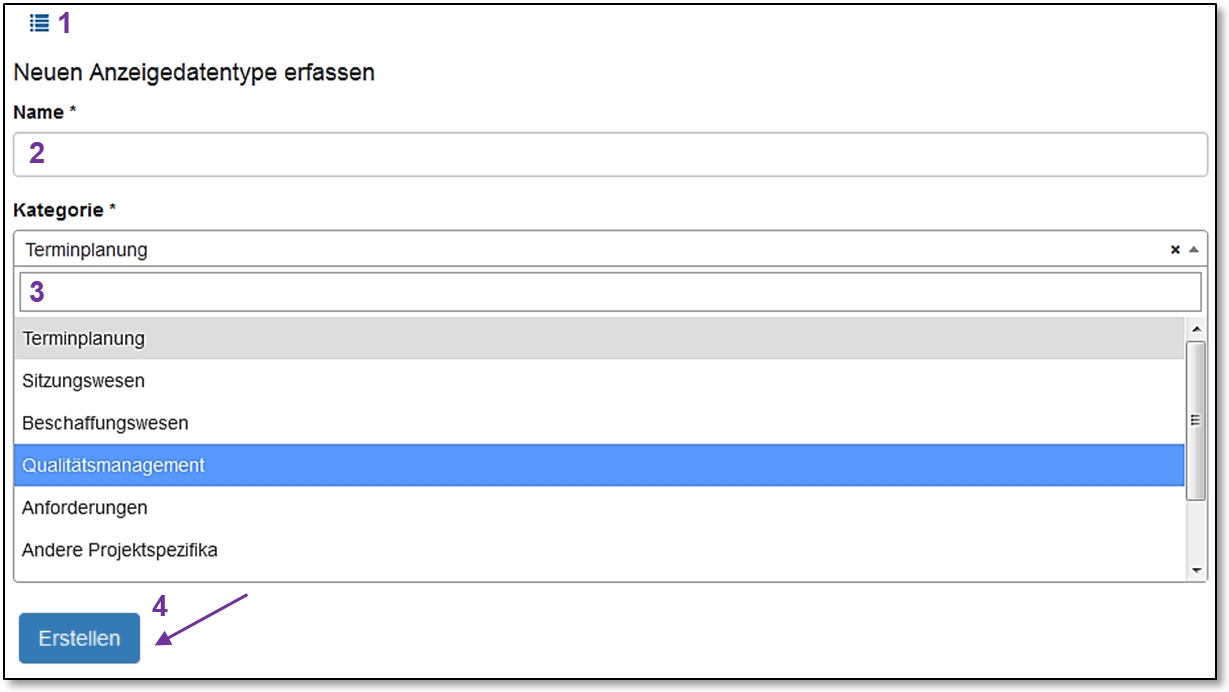
\includegraphics[width=1\linewidth]{../chapters/09_Qualitaetsmanagement/pictures/9-1-1_Anzeigedatentypen_Eingaben.jpg}}
\caption{Anzeigedatetypen erstellen }
% \label{fig:speciation}
\end{figure}

Mit dem Listensymbol 
\includegraphics[height=12pt]{/Icons/Listensymbol_zurueck.jpg} \col{(1)} kehren Sie zur Übersicht zurück. Geben Sie einen aussagekräftigen Namen für die Dokumentenverknüpfung ein \col{(2)} (Dieser Name erscheint dann im CUBE PA Menü). Wählen Sie unter 'Kategorie' \col{(3)} im Dropdownmenü den Punkt 'Qualitätsmanagement' aus und klicken Sie anschliessend 'Erstellen'. Die Daten werden gespeichert.

\vspace{\baselineskip}

\textbf{2. Schritt: 'Anzeigedaten' erstellen}

Nun legen Sie den Eintrag an, welcher auch das verknüpfte Dokument enthält. Dazu gehen Sie im Menü links zum Punkt 'Konfigurationen' und dem Unterpunkt 'Anzeigedaten'. Folgende Übersicht wird geöffnet: 

\begin{figure}[H]
\center{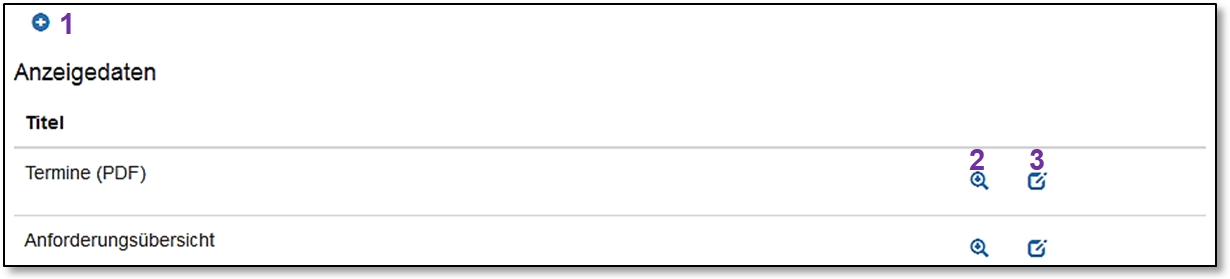
\includegraphics[width=1\linewidth]{../chapters/09_Qualitaetsmanagement/pictures/9-1-1_Anzeigedaten_Uebersicht.jpg}}
\caption{Anzeigedaten Übersicht}
% \label{fig:speciation}
\end{figure}

Mit dem Plussymbol 
\includegraphics[height=12pt]{/Icons/Plussymbol.jpg} \col{(1)} legen Sie einen neuen Eintrag an. Mit dem Lupensymbol 
\includegraphics[height=12pt]{/Icons/Lupe.jpg} \col{(2)} oder dem Bearbeitungssymbol 
\includegraphics[height=12pt]{/Icons/Bearbeiten.jpg} \col{(3)} können Sie einen bestehenden Eintrag anschauen oder bearbeiten. Mit Klick auf das Plussymbol 
\includegraphics[height=12pt]{/Icons/Plussymbol.jpg} \col{(1)} wird nun eine neue Dokumentenverknüpfung erstellt. 

\begin{figure}[H]
\center{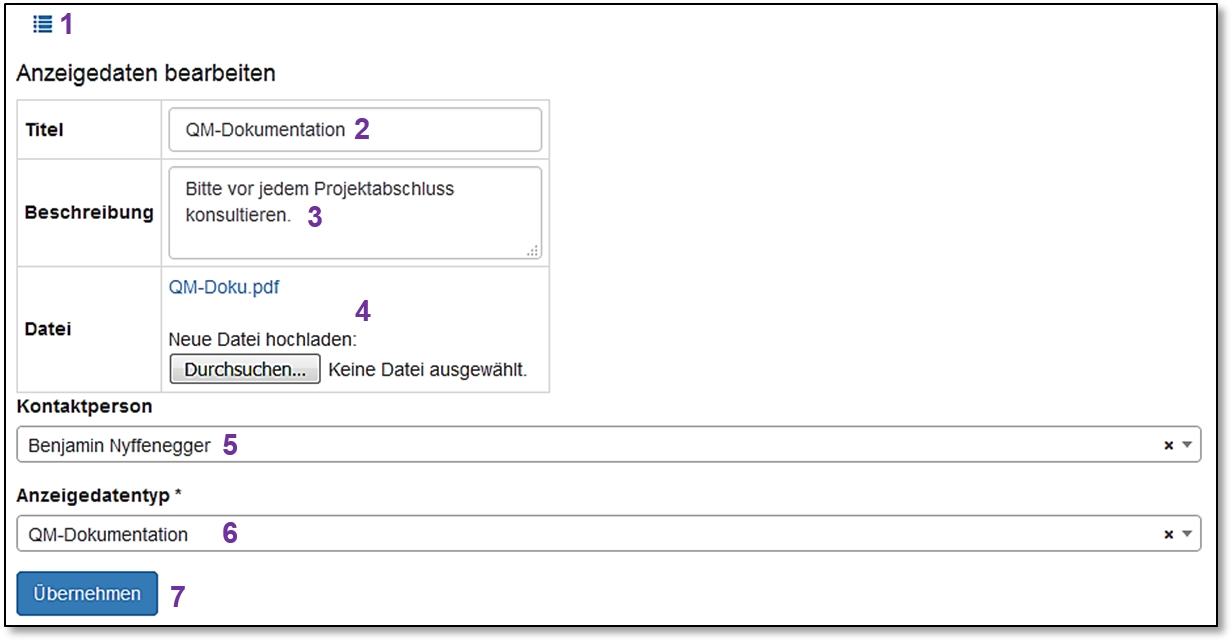
\includegraphics[width=1\linewidth]{../chapters/09_Qualitaetsmanagement/pictures/9-1-1_Anzeigedaten_Eingaben.jpg}}
\caption{Anzeigedaten erstellen}
% \label{fig:speciation}
\end{figure}

Mit dem Listensymbol 
\includegraphics[height=12pt]{/Icons/Listensymbol_zurueck.jpg} \col{(1)} kehren Sie zur Übersicht zurück. Geben Sie nun einen gewünschten Titel \col{(2)} ein (allenfalls derselbe wie Sie den 'Anzeigedatentyp' benannt haben. Sie können nun eine Beschreibung \col{(2)} einfügen, welche dann unter 'Qualitätsmanagement' und dem entsprechenden / erstellten Menüpunkt angezeigt wird. Nun wird unter Datei \col{(4)} das gewünschte Dokument hochgeladen und verknüpft. Klicken Sie auf 'Durchsuchen' und wählen Sie anschliessend im Explorer-Fenster die benötigte Datei aus.\\

Optional können Sie eine Kontaktperson \col{(5)} auswählen. Diese wird dann ebenfalls und mit der hinterlegten Email-Adresse angezeigt. Nun werden die 'Anzeigedaten' mit dem gewünschten 'Anzeigedatentyp' verknüpft \col{(6)}. Abschliessend klicken Sie auf 'Übernehmen', die Daten werden gespeichert. Die Vorbereitungsarbeiten sind nun gemacht, die verknüpfte Datei kann nun unter 'Qualitätsmanagement' und dem entsprechenden Unterpunkt geöffnet werden. Zur besseren Übersicht, welche Daten angezeigt werden hier nochmals der Dokumenteneintrag mit Kommentaren:

\begin{figure}[H]
\center{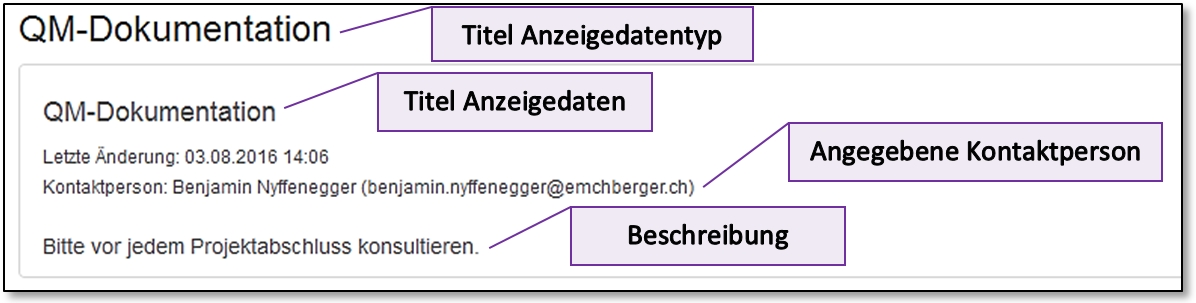
\includegraphics[width=1\linewidth]{../chapters/09_Qualitaetsmanagement/pictures/9-1-1_AngezeigteDaten.jpg}}
\caption{Anzeigedatentypen unter Qualitätsmanagement}
% \label{fig:speciation}
\end{figure}

Wenn sich das verknüpfte Dokument ändert, können Sie den bestehenden Eintrag bearbeiten und einfach die neue Datei hochladen. Die 'Letzte Änderung' wird somit aktualisiert und die neue Datei steht zur Verfügung.

\subsection{Projekthandbuch}

\begin{wrapfigure}[6]{l}{6.5cm}   % [x] Wie manche Zeile soll sich um die Grafik "brechen"
  \vspace{-35pt}      % Grundwert war 20; mit 30 schön oben beim Text ausgerichtet
  \begin{center}
    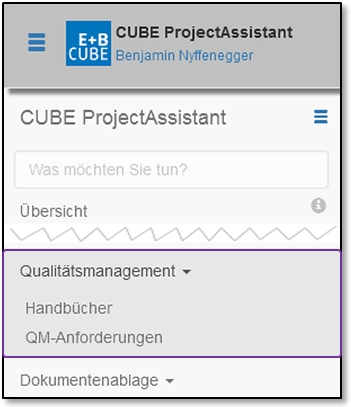
\includegraphics[width=1\linewidth]{../chapters/09_Qualitaetsmanagement/pictures/9-2_Menu_Qualitaetsmanagement_Handbuch.jpg}
  \end{center}
  \vspace{-20pt}
  \caption{Die Funktion Handbuch im CUBE PA}
  \vspace{-10pt}
\end{wrapfigure}

Innerhalb des Qualitätsmanagements können Sie Handbücher, wie zum Beispiel ein Projekthandbuch, entwerfen. Wählen Sie dazu den Unterpunkt 'Handbücher'. 

\vspace{2.5cm}  

Haben Sie bereits Handbücher erfasst, werden diese auf folgender Übersicht aufgeführt:

\vspace{3cm}  

\begin{figure}[H]
\center{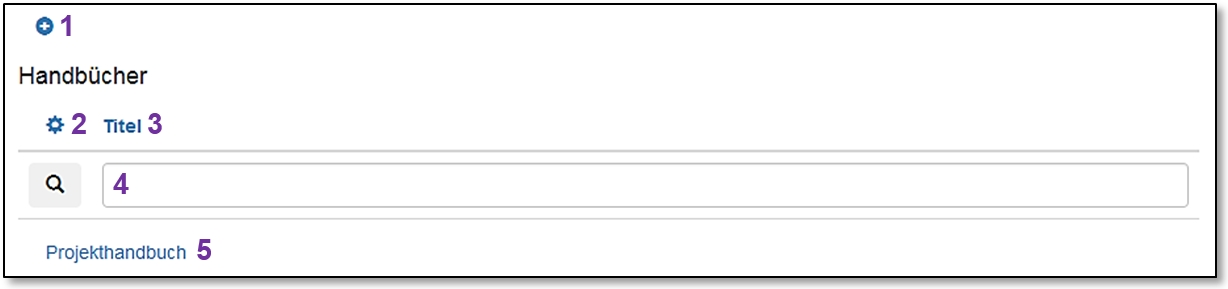
\includegraphics[width=1\linewidth]{../chapters/09_Qualitaetsmanagement/pictures/9-2_Handbuch_Uebersicht.jpg}}
\caption{Übersicht über die Handbücher}
% \label{fig:speciation}
\end{figure}

Mit dem Plussymbol 
\includegraphics[height=12pt]{/Icons/Plussymbol.jpg} \col{(1)} können Sie ein weiteres Handbuch erfassen (siehe Kapitel \ref{bkm:Ref930000788}). Mit dem Konfigurationssymbol 
\includegraphics[height=12pt]{/Icons/SpaltenEinst.jpg} \col{(2)} können Spalten ein- und ausgeblendet werden (In diesem Fenster können Sie aktuell keine Änderungen vornehmen, da es nur eine Spalte gibt). Mit Klick auf den blauen Titel \col{(3)} können Sie die angezeigten Handbücher von A bis Z oder Z bis A sortieren. Wollen Sie nach einem bestimmten Handbuch suchen, können Sie in die Suchzeile \col{(4)} einen beliebigen Begriff eingeben und anschliessend die Lupe 
\includegraphics[height=12pt]{/Icons/Lupe_s.jpg} oder die 'Enter-Taste' drücken. Anschliessend erhalten Sie die gefilterte Dokumenten-, respektive Handbuchliste. (Achtung: Aktuell funktioniert der Filter nur hinsichtlich den Handbuchtiteln und nicht auf deren Inhalt). Klicken Sie auf ein Hanbuch \col{(5)}, um dieses zu öffnen:

\begin{figure}[H]
\center{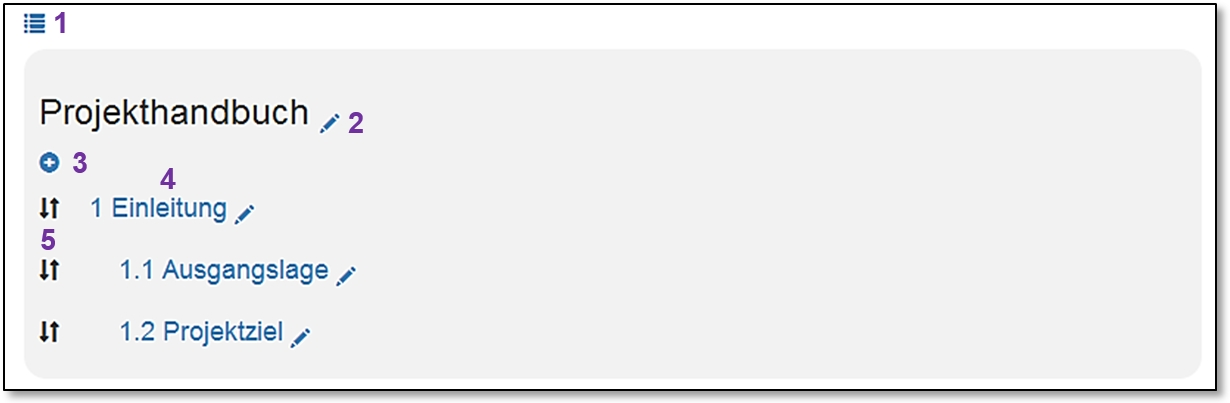
\includegraphics[width=.75\linewidth]{../chapters/09_Qualitaetsmanagement/pictures/9-2_Projekthandbuch.jpg}}
\caption{Ein Handbuch im Überblick}
% \label{fig:speciation}
\end{figure}

Mit dem Listensymbol 
\includegraphics[height=12pt]{/Icons/Listensymbol_zurueck.jpg} \col{(1)} können Sie wieder auf die Übersicht der Handbücher zurückkehren. Sie sehen nun das Handbuch in der Übersicht. Mit dem Stiftsymbol 
\includegraphics[height=12pt]{/Icons/Stift.jpg} \col{(2)} können Sie jeweils den Eintrag bearbeiten und mit dem Plussymbol 
\includegraphics[height=12pt]{/Icons/Plussymbol.jpg} \col{(3)} ein neues Kapitel anlegen. Wenn Sie auf einen blauen Titel klicken \col{(4)} wird dieses Kapitel geöffnet. Soll die Reihenfolge geändert werden, packen Sie die vertikalen Pfeile 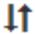
\includegraphics[height=12pt]{/Icons/VertPfeile.jpg} \col{(5)} vor einem Kapitel mit der linken Maustaste (klicken und gedrückt halten) und schieben diese nach oben oder unten an die gewünschte Position. \\
Sie haben die Möglichkeit, das ganze Handbuch als pdf-Dokument zu speichern. Klicken Sie dazu auf das Download-Symbol 
\includegraphics[height=12pt]{/Icons/Download.jpg} \col{(6)}. Beim Speichervorgang wird ein zip-Ordner angelegt, welcher das pdf-Handbuch und zusätzlich die im Dokument enthaltenen, resp. eingebundenen Dokumente enthält.

\subsubsection{Ein bestehendes Handbuch ändern}

Der Titel eines Handbuchs wird gerade in der Übersicht geändert (Klick auf den Stift 
\includegraphics[height=12pt]{/Icons/Stift.jpg} \col{(2)}). Nach der Änderung klicken Sie auf das kleine Gutzeichen hinter dem Titel. Die Änderung ist gespeichert:

\begin{figure}[H]
\center{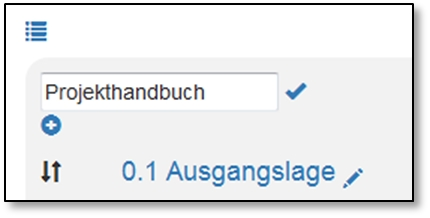
\includegraphics[width=0.35\linewidth]{../chapters/09_Qualitaetsmanagement/pictures/9-2-1_HandbuchTitel_aendern.jpg}}
\caption{Titel eines Handbuches ändern}
% \label{fig:speciation}
\end{figure}

Wenn Sie einen Eintrag ändern wollen, klicken Sie auf das Stiftsymbol 
\includegraphics[height=12pt]{/Icons/Stift.jpg} hinter dem gewünschten Kapitel. Folgende Eingabemaske erscheint:

\begin{figure}[H]
\center{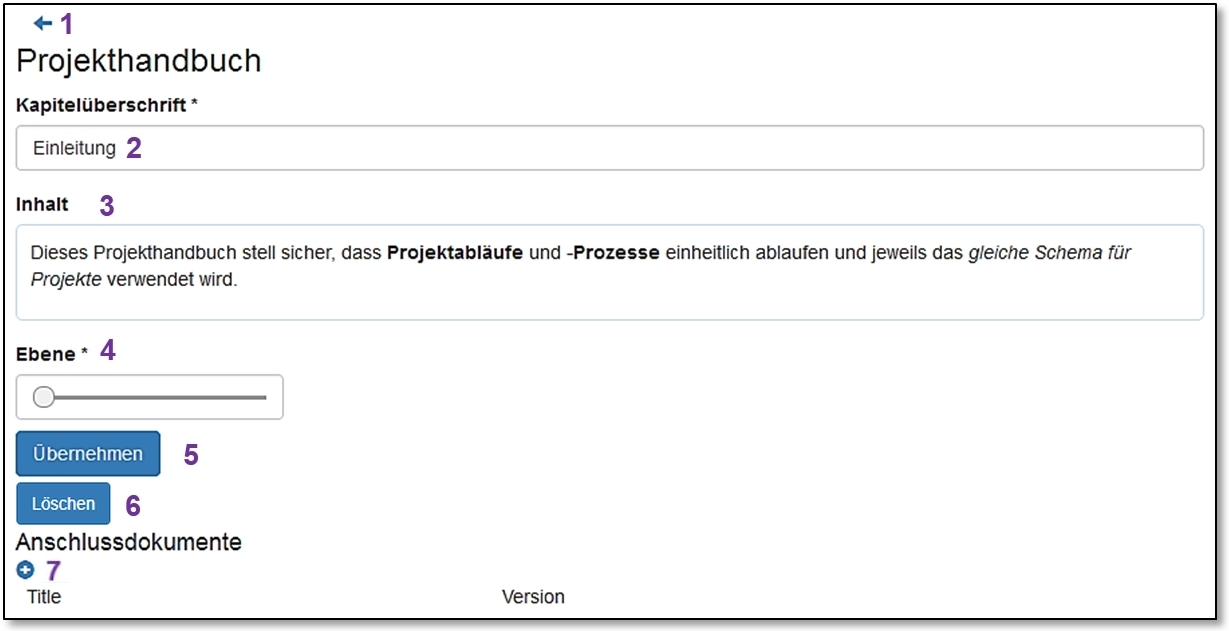
\includegraphics[width=1\linewidth]{../chapters/09_Qualitaetsmanagement/pictures/9-2-1_Handbuch_aendern.jpg}}
\caption{Ein Kapitel ändern}
% \label{fig:speciation}
\end{figure}

Mit dem Pfeil-Symbol 
\includegraphics[height=12pt]{/Icons/Pfeil-links.jpg} \col{(1)} können Sie wieder zum Handbuch (Übersicht) zurückkehren. In den verschiedenen Eingabefeldern sehen Sie die bestehenden Einträge, welche nun geändert werden können. Unter Kapitelüberschrift \col{(2)} können Sie den Kapiteltitel ändern (dies ist ein Pflichtfeld und muss ausgefüllt sein / bleiben, unter Inhalt \col{(3)} wird der Inhalt des Kapitels geändert. Mit dem Ebene-Regler \col{(4)} können Sie die Hierarchie / Gliederung des Kapitels beeinflussen. Für die erste Hierarchie (1) stellen Sie den Regler ganz nach links, die Mittelposition bedeutet die erste Unterebene (1.1) und die rechte Position die zweite Unterebene (1.1.1). \\
Löschen Sie ein überzähliges Kapitel mit Klick auf den 
\includegraphics[height=14pt]{/Icons/B_Loeschen.jpg}-Button \col{(6)}.
Den einzelnen Kapitel können Dokumente zugeordnet werden. Mit dem Plussymbol 
\includegraphics[height=12pt]{/Icons/Plussymbol.jpg} \col{(7)} gelangen Sie zur Anschlussdokumenten-Übersicht:

\begin{figure}[H]
\center{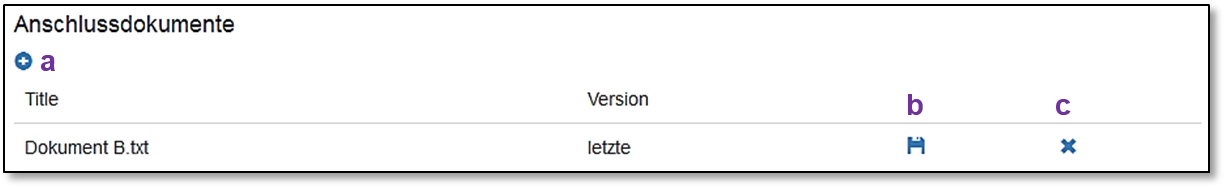
\includegraphics[width=1\linewidth]{../chapters/09_Qualitaetsmanagement/pictures/9-2-1_Anschlussdokumente_aendern.jpg}}
\caption{Anschlussdokumente}
% \label{fig:speciation}
\end{figure}

Mit dem Plussymbol 
\includegraphics[height=12pt]{/Icons/Plussymbol.jpg} \col{(a)} können Sie ein weiteres Dokument hinzufügen. Ein bestehendes Dokument lässt sich mittels dem Speichern-Symbol 
\includegraphics[height=12pt]{/Icons/Diskette.jpg} \col{(b)} auf dem Computer abspeichern oder mit dem Kreuzchen 
\includegraphics[height=12pt]{/Icons/Kreuzchen.jpg} \col{(c)} löschen.

Sämtliche Änderungen müssen mit 'Übernehmen' \col{(5)} gespeichert werden. 

\subsubsection{Ein neues Handbuch erstellen}
\label{bkm:Ref930000788}

Wenn Sie ein neues Handbuch erstellen wollen, gehen Sie wie folgt vor:

Im Menü links wählen Sie den Punkt 'Qualitätsmanagement' und den Unterpunkt 'Handbücher'. Klicken Sie in der Handbuchübersicht auf das Plussymbol 
\includegraphics[height=12pt]{/Icons/Plussymbol.jpg} \col{(1)}.

\begin{figure}[H]
\center{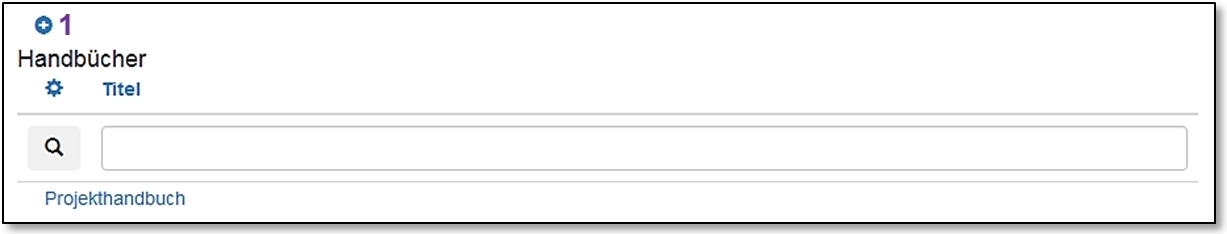
\includegraphics[width=1\linewidth]{../chapters/09_Qualitaetsmanagement/pictures/9-3-2_NeuesHandbuch_erstellen.jpg}}
\caption{Neues Handbuch erstellen}
% \label{fig:speciation}
\end{figure}

Geben Sie nun einen passenden Titel für das neue Handbuch ein: 

\begin{figure}[H]
\center{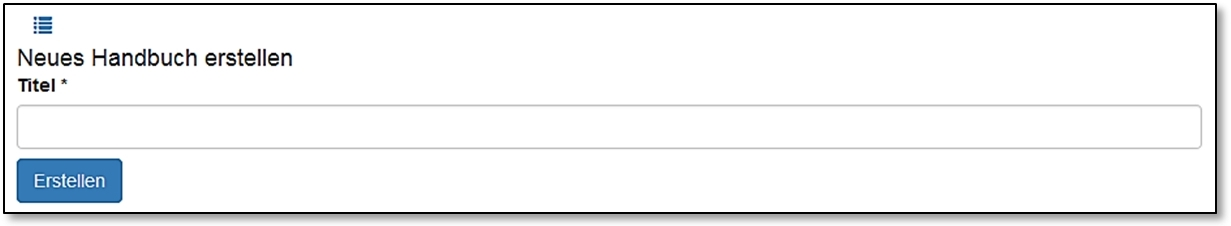
\includegraphics[width=1\linewidth]{../chapters/09_Qualitaetsmanagement/pictures/9-3-2_Handbuch_erstellen_Titel.jpg}}
\caption{Neues Handbuch erstellen - Titel eingeben}
% \label{fig:speciation}
\end{figure}

Anschliessend klicken Sie auf den 'Erstellen'-Button. Das Handbuch wird nun angelegt.

\begin{figure}[H]
\center{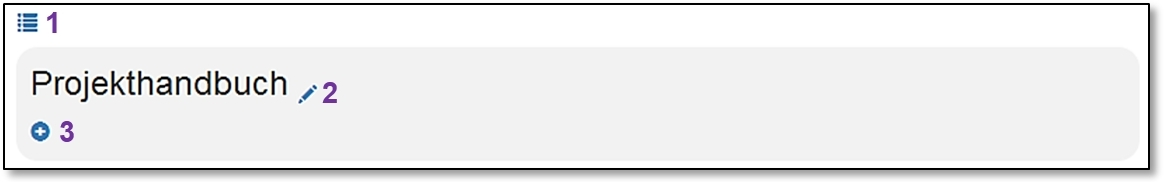
\includegraphics[width=.8\linewidth]{../chapters/09_Qualitaetsmanagement/pictures/9-3-2_Handbuch_angelegt.jpg}}
\caption{Neues Handbuch - Kapitel anlegen}
% \label{fig:speciation}
\end{figure}

Das Handbuch wurde nun angelegt. Mittels dem Listensymbol 
\includegraphics[height=12pt]{/Icons/Listensymbol_zurueck.jpg} \col{(1)} gelangen Sie jeweils wieder zur Übersicht der Handbücher. Mit dem Stiftsymbol 
\includegraphics[height=12pt]{/Icons/Stift.jpg} \col{(2)} können Sie den Titel wieder ändern. Mit dem Plussymbol 
\includegraphics[height=12pt]{/Icons/Plussymbol.jpg} \col{(3)} werden nun Kapitel angelegt:

\begin{figure}[H]
\center{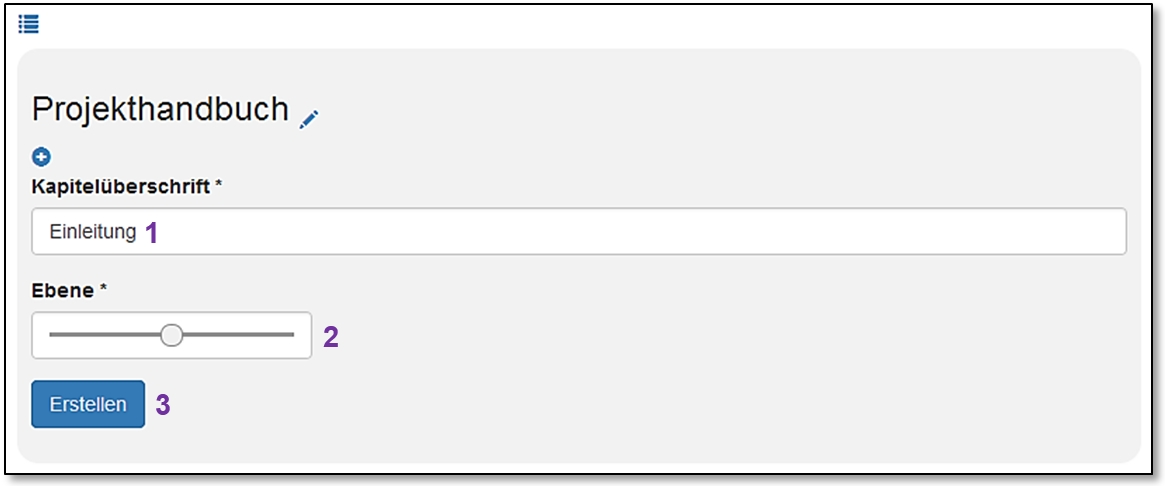
\includegraphics[width=.8\linewidth]{../chapters/09_Qualitaetsmanagement/pictures/9-3-2_Kapitel_anlegen.jpg}}
\caption{Neues Handbuch - Kapitel benennen}
% \label{fig:speciation}
\end{figure}

Geben Sie die gewünschte Kapitelüberschrift ein \col{(1)}. Sie haben nun die Möglichkeit bereits die Gliederung einzustellen (Links: 1, Mitte: 1.1, Rechts: 1.1.1). Sie können diese Gliederung selbstverständlich später verändern. Haben Sie die gewünschten Eingaben und Einstellungen vorgenommen, klicken Sie auf 'Erstellen'. Das Kapitel wird nun angelegt und die Eingabe-Maske ändert sich:

\begin{figure}[H]
\center{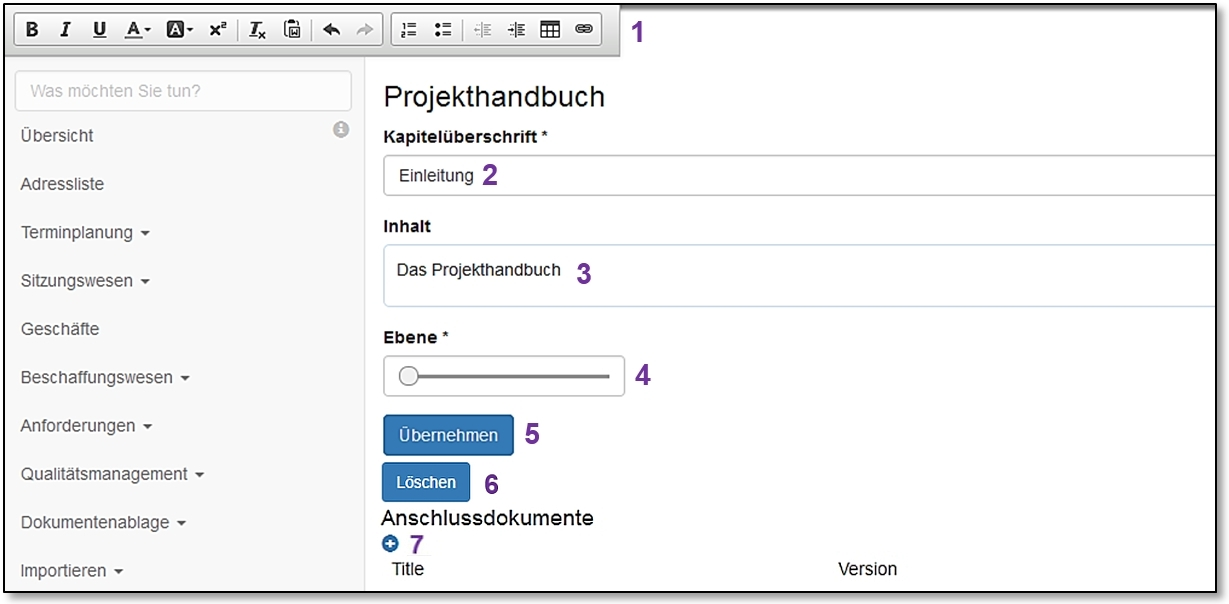
\includegraphics[width=1\linewidth]{../chapters/09_Qualitaetsmanagement/pictures/9-2-3_Kapitel_bearbeiten.jpg}}
\caption{Neues Handbuch - Kapitel bearbeiten}
% \label{fig:speciation}
\end{figure}

Sie können nach wie vor die Kapitelüberschrift verändern. \col{(2)}. Wenn Sie in das Feld 'Inhalt' \col{(3)} klicken, wird oben links im Bild ein 'Funktionsmenü' angezeigt \col{(1)}. Mit diesen Funktionen haben Sie die Möglichkeit den Text zu formatieren, Tabellen zu erstellen oder Änderungen rückgängig zu machen. Mehr dazu weiter unten. Ebenfalls können Sie an dieser Stelle mit dem Ebene-Regler \col{(4)} die Textgliederung weiterhin anpassen. Alle Änderungen müssen mit dem Button 'Übernehmen' \col{(5)} gespeichert werden. Mit Klick auf den 
\includegraphics[height=14pt]{/Icons/B_Loeschen.jpg}-Button \col{(6)} können Sie ein Kapitel wieder löschen. Nun erscheint eine weitere Option: Sie können in jedem Kapitel Dokumente hinzufügen, respektive verlinken \col{(7)}. Dazu klicken Sie auf das Plussymbol 
\includegraphics[height=12pt]{/Icons/Plussymbol.jpg} \col{(7)}. Nun kann ein oder können mehrere Dokument/e verknüpft werden:

\begin{figure}[H]
\center{\includegraphics[width=1\linewidth]{../chapters/09_Qualitaetsmanagement/pictures/9-3-2_Kapitel_Dokumente_hinzufuegen.jpg}}
\caption{Neues Handbuch - Dokumente hinzufügen}
% \label{fig:speciation}
\end{figure}

Während dem Erstellen oder beim Bearbeiten eines Handbuches können Sie jeweils mit dem Pfeilsymbol \includegraphics[height=12pt]{/Icons/Pfeil-links.jpg} \col{(1)} zurück zur Buchübersicht / -gliederung wechseln. Bitte beachten Sie, dass jedoch Ihre Änderungen verloren gehen, wenn Sie nicht vorher den 'Übernehmen'-Button gedrückt haben. Befinden Sie sich im Textfeld 'Inhalt', wird das Pfeilsymbol überdeckt. Klicken Sie beispielsweise in die Kapitelüberschrift, damit der Funktionsbalken verschwindet und das Pfeilsymbol sichtbar wird. \\

\textbf{Dokumente verknüpfen:} Unten im Fenster haben Sie nun die Möglichkeit, ein Dokument auszuwählen und dieses mit dem Kapitel zu verknüpfen. Es stehen Ihnen sämtliche Dokumente zu Verfügung, welche Sie in der Dokumentenablage des CUBE PA hochgeladen haben. Falls Sie während dem Bearbeiten eines Handbuches ein neues Dokument verknüpfen wollen, müssen Sie Ihre aktuelle Arbeit mittels 'Übernehmen'-Button speichern und dann unter Dokumentenablage links im Hauptmenü das gewünschte Dokument im CUBE PA zuerst erfassen. Mehr zum Thema 'Dokumente hochladen' finden Sie im Kapitel \ref{bkm:Ref442863508}. \\

Mit der Funktion 'Dokumentenversion explizit festlegen' \col{(2)} haben Sie die Möglichkeit, eine bestimmte Version eines Dokumentes zu verknüpfen. Falls Sie die Funktion nicht anwählen, wird im Kapitel des Handbuches immer die aktuellste Version, welche in der Dokumentenablage hochgeladen wurde, angezeigt/verknüpft. Es kann Situationen geben, welche erfordern, dass eine bestimmte Version eines Dokumentes verknüpft bleibt. Klicken Sie dazu in das kleine Rechteck; die Funktion wird aktiviert. Mehr zum Thema Dokumentenablage und den verschiedenen Versionen finden Sie im Kapitel \ref{bkm:Ref443047930}. \\

Wenn Sie mehrere Dokumente verknüpfen wollen wiederholen Sie obige Schritte. \\

\pagebreak
\textbf{Text formatieren und weitere Funktionen:}

\begin{figure}[H]
\center{\includegraphics[width=.8\linewidth]{../chapters/09_Qualitaetsmanagement/pictures/9-2-3_Text_formatieren.jpg}}
\caption{Neues Handbuch - Text formatieren.}
% \label{fig:speciation}
\end{figure}

Ähnlich wie bei einer Textverarbeitungssoftware haben Sie die Möglichkeit den Kapitelinhalt zu formatieren, Tabellen oder Links zu Webseiten einzufügen. Im Folgenden finden Sie eine Übersicht über die verschiedenen Funktionen: \\

\begin{tabular}{c | p{14cm} l} %{cl}
\hline
\includegraphics[height=12pt]{../chapters/09_Qualitaetsmanagement/pictures/Format/Fett.jpg} & Der Text wird fett dargestellt \\
\hline
\includegraphics[height=12pt]{../chapters/09_Qualitaetsmanagement/pictures/Format/Kursiv.jpg} & Der Text wird kursiv dargestellt \\
\hline
\includegraphics[height=12pt]{../chapters/09_Qualitaetsmanagement/pictures/Format/Unterstrichen.jpg} & Der Text wird unterstrichen dargestellt \\
\hline
\includegraphics[height=12pt]{../chapters/09_Qualitaetsmanagement/pictures/Format/Textfarbe.jpg} & Die Textfarbe kann damit geändert werden \\
\hline
\includegraphics[height=12pt]{../chapters/09_Qualitaetsmanagement/pictures/Format/Hintergrundfarbe.jpg} & Die Hintergrundfarbe des Textes kann damit geändert werden \\
\hline
\includegraphics[height=12pt]{../chapters/09_Qualitaetsmanagement/pictures/Format/Form_z.jpg} & Mit dieser Funktion kann die Formatierung zurückgesetzt werden \\
\hline
\includegraphics[height=12pt]{../chapters/09_Qualitaetsmanagement/pictures/Format/ausWord.jpg} & Mit dieser Funktion kann ein Inhalt z.B. aus Word eingefügt werden, welcher sich in der Zwischenablage befindet. (Falls der Browser diese Funktionalität nicht unterstützt, erscheint eine entsprechende Meldung. Sie haben nun aber trotzdem die Möglichkeit, den zwischengespeicherten Text in der erscheinenden Box einzufügen und somit in CUBE PA zu übertragen.) \\
\hline
\includegraphics[height=12pt]{../chapters/09_Qualitaetsmanagement/pictures/Format/Undo.jpg} & Änderungen lassen sich mit der 'Undo' oder 'Redo' Funktion rückgängig machen oder wiederherstellen \\
\hline
\includegraphics[height=12pt]{../chapters/09_Qualitaetsmanagement/pictures/Format/Aufzaehlung.jpg} & Es besteht die Möglichkeit Aufzählungen mittels Nummerierung oder einem Punkt einzufügen \\
\hline
\includegraphics[height=12pt]{../chapters/09_Qualitaetsmanagement/pictures/Format/Einruecken.jpg} & Mit dieser Funktion lässt sich der gewünschte Text nach rechts einrücken oder wiederum nach links zu verschieben \\
\hline
\includegraphics[height=12pt]{../chapters/09_Qualitaetsmanagement/pictures/Format/Tabellen.jpg} & Es können Tabellen eingefügt werden. Die Tabellen können beschriftet und formatiert werden (Rahmen, Grösse, Ausrichtung etc.) \\
\hline
\includegraphics[height=12pt]{../chapters/09_Qualitaetsmanagement/pictures/Format/Link.jpg} & Mit dieser Funktion können Links auf Webseiten oder Textmarker innerhalb des Textes (Handbuch) gemacht, respektive verknüpft werden. Auch Email-Adressen können auf diese Weise im Handbuch eingebunden werden. \\
\hline
\end{tabular}

\vspace{\baselineskip}

\textbf{Hinweis:} Sie können formatierte Textblöcke aus einem Word oder einer Internetquelle kopieren und in das Handbuch / den Inhalt kopieren. Die Formatierung wird dabei übernommen. Dies gilt auch für Links.




